\chapter{Orderbook Trading Simulator}
\label{chap:simulator}
This chapter describes the \ac{OTS} and it's underlying OrderbookContainers, implemented within the scope of this thesis. Fed with historic orderbook data it serves as a backtesting framework for testing out various trading strategies. The \ac{OTS} provides detailed feedback in terms of trading progress, achieved prices and accrued costs.

\section{Data Origin}
\label{chap:dataorigin}
Since typical financial data providers must make an earning from their treasures, they typically only deliver delayed market data on a complimentary basis. Investors dependent on real time or level 2 market data (see \Cref{sec:marketdata:levels}) are usually charged horrendous monthly subscription fees.\\

A costless alternative exists in open cryptocurrencies, like bitcoins (see \Cref{chap:bitcoins}). The digital asset exchange platform Poloniex \cite{poloniex} provides an open API for querying detailed market data in real time. As their push API, to receive live order book updates and trades, was rather error-prone and buggy when this project started, the decision was made, to query full orderbooks on a minutely basis.\\

On Nov, 10th 2016, 10:00 am, a daemon was started, to fetch orderbook snapshots up to a market depth of 5000 from Poloniex via HTTP GET requests (see \Cref{lst:PoloniexFetch}). The volume of recorded orderbook snapshots for nine distinct currency pairs\footnote{Recorded currency pairs include USDT/BTC, BTC/ETH, BT/XMR, BTC/XRP, BTC/FCT, BTC/NAV, BTC/DASH, BTC/MAID, BTC/ZEC} has since grown to roughly 100GB (as per 2017-06-20). This thesis is based on a condensed version of the currency pair USDT/Bitcoin.

\begin{lstlisting}[frame=single, breaklines=true, basicstyle=\scriptsize, caption=Data fetched from Poloniex via HTTP GET request, label=lst:PoloniexFetch]
# https://poloniex.com/public?command=returnOrderBook&currencyPair=USDT_BTC&depth=5000
{"asks" :[[ "705.450000" ,2.772181], [ "705.450196", 0.139212] ,["706.170000" ,0.052838] , ... ], "bids":[["705.000000",0.158232],["703.700000" ,0.001250], ... ], "isFrozen": 0, "seq": 63413296}
\end{lstlisting}

\begin{figure}[ht]
	\centering
   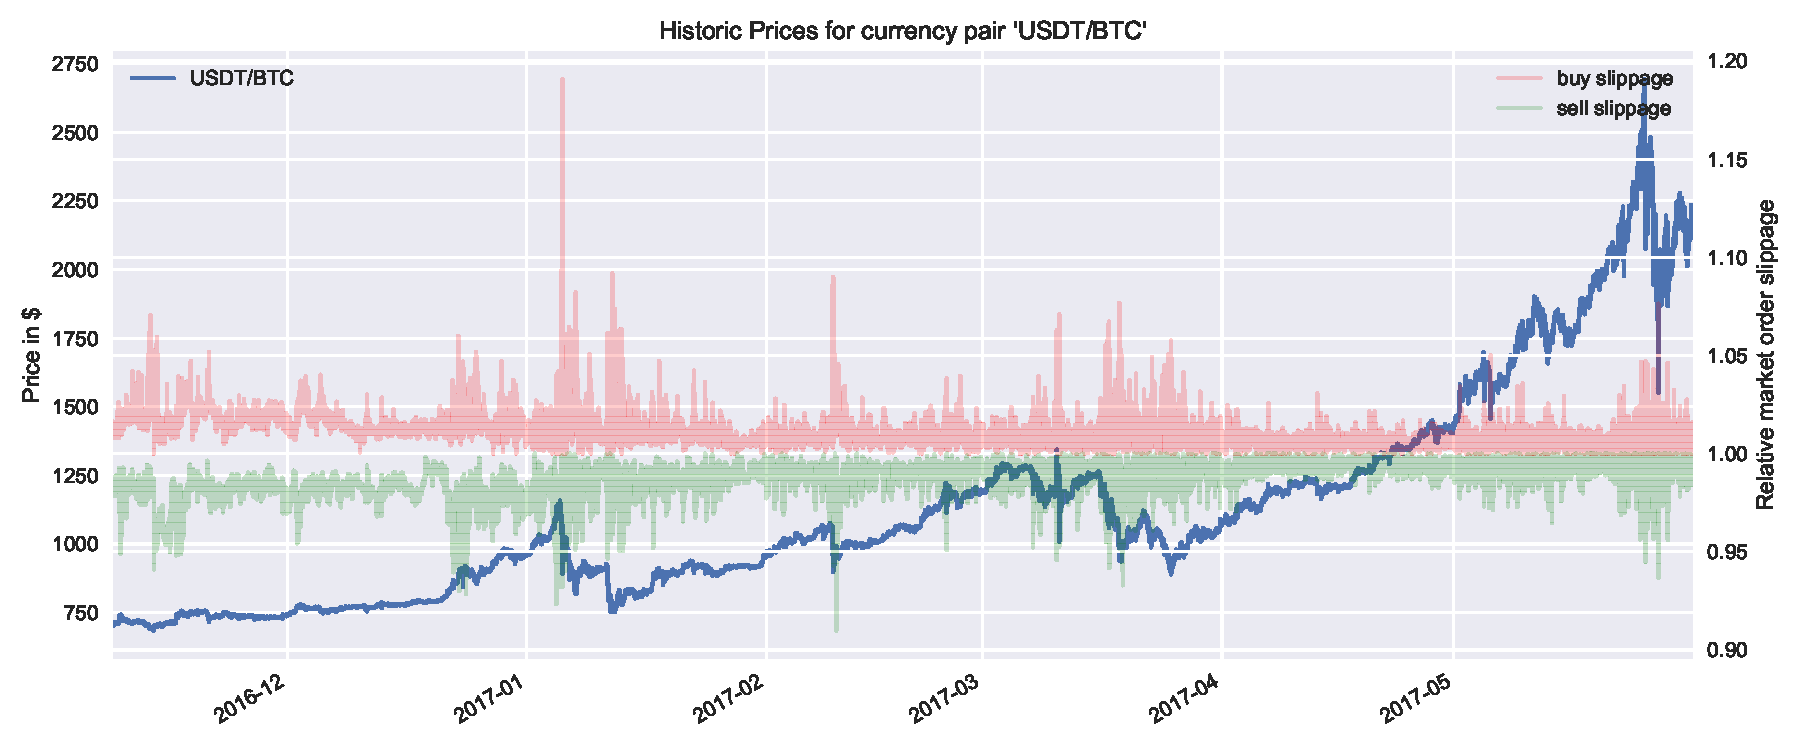
\includegraphics[width=1.\textwidth]{content/drawings/bitcoin_historicPrices}
	\caption{Historic center prices between Nov, 10th 2016 and May, 31 2017, as fetched from Poloniex.}
	\label{fig:ploniexPriceHistory}
\end{figure}

\Cref{fig:ploniexPriceHistory} shows the price evolution of currency pair USDT/Bitcoin over the period of recording. Prices have burst from roughly 700\$ to more than 2.000\$. Red and green lines depict the relative difference between the worst price paid/received for an immediate market orders of $70.000\$$, respectively.

\section{Data preprocessing}
\label{chap:preprocessing}
The python \lstinline!class OrderbookContainer! aggregates all informations contained in an individual orderbook snapshot. It enforces correct price ordering in the two opposing bid and ask books and provides additional methods for market visualization and feature extraction. To restrict wasteful memory usage, orderbook snapshots are condensed in several ways:

\begin{itemize}
\item Almost identically price levels are round to the second decimal and their respective order volumes merged.

 \[ 
  \begin{rcases}
    0.139212 * 705.450000\\
    2.632969 * 705.450196\\
  \end{rcases} 
  = 2.772181 * 705.45
\]
\item Market depth is capped just above the threshold of 100 bitcoins, roughly corresponding to a market depth of 100-140 prices levels in both books. This threshold allows to simulate trades up to a market order price of 70.000 \$ at any time throughout the whole recording period.

\item Erroneous orderbook snapshots have been discarded. Occasional errors may occur, due to Poloniex API failures.

\end{itemize}

These measurements reduce the average individual orderbook snapshots size from 30KB to approximately 6.6KB. As for the december 2016, this results into 44.640 snapshots with a total size of 295MB instead of 1.35GB, clearly reducing the memory consumption.\\

\Cref{lst:OrderbookContainer} shows the most important functions, provided by the OrderbookContainer class. OrderbookContainer instances are vigorously used by the \ac{OTS}. \Cref{fig:orderbook} shows a plain visualization of an individual orderbook snapshot.

\begin{lstlisting}[frame=single, breaklines=true, basicstyle=\scriptsize, caption=OrderbookContainer, label=lst:OrderbookContainer]
ob = OrderbookContainer(timestamp="2016-11-08T10:00",
                        bids=pd.DataFrame([200., 100., 300.],
                        columns=['Amount'], index=[28.7, 28.5, 28]),
                        asks=pd.DataFrame([25., 50., 200.],
                        columns=['Amount'], index=[29., 30., 31.]))
# Available methods
ob.plot(outfile='sample.pdf')  # plt.show or plt.savefig
ob.asks  # pd.DataFrame
ob.bids  # pd.DataFrame
ob.features  # returns a dict of precomputed features
ob.get_bid(), ob.get_ask(), ob.get_center()  # float
ob.get_current_price(volume=100)  # achievable cashflow by market order
ob.get_current_sharecount(cash=70000) # number of shares aquirable by market order
ob.compare_with(other_ob) # returns orderbook deltas used by the OTS
ob.enrich()  # computes Volume, VolumeAcc and norm_Price
ob.head(depth=3)  # returns the orderbook, capped at a market depth of 3
ob.plot()
\end{lstlisting}


\begin{figure}[ht]
	\centering
   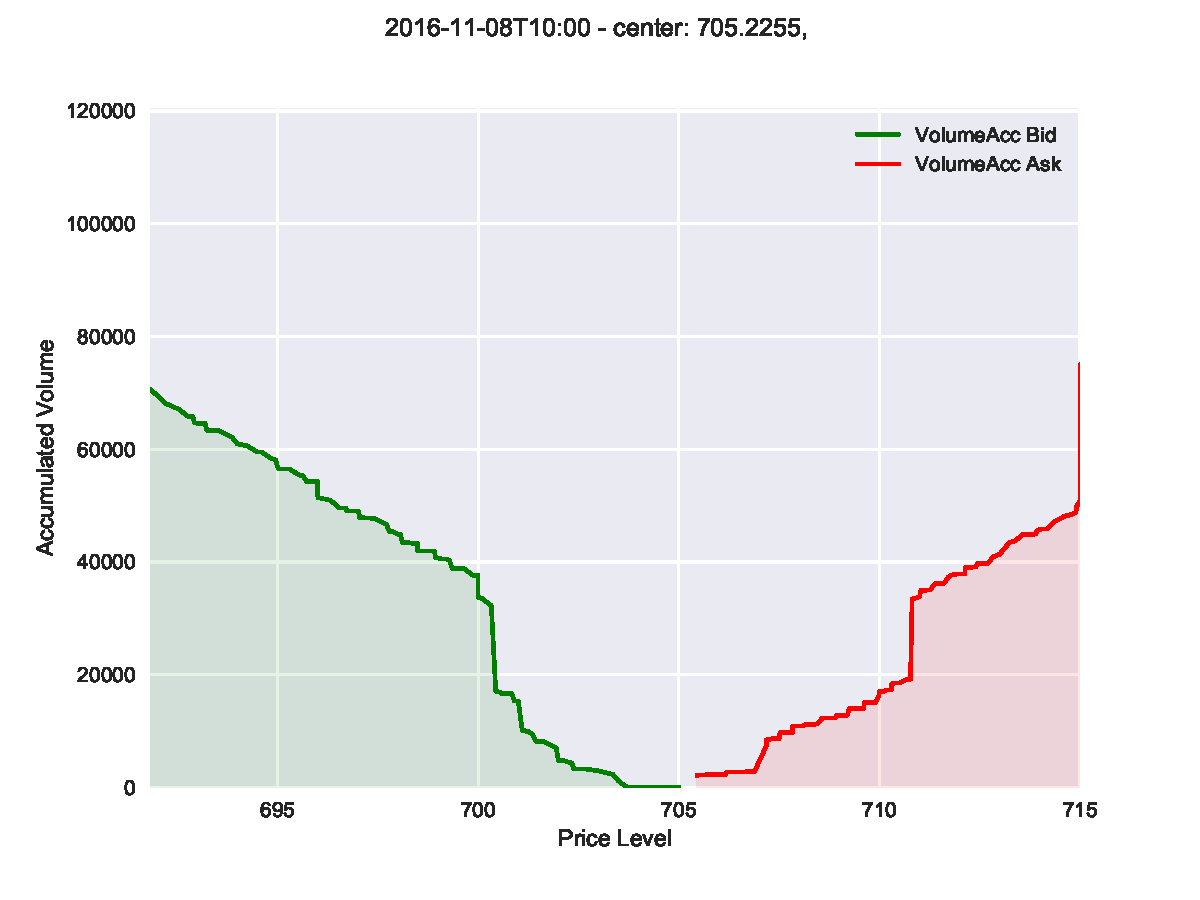
\includegraphics[width=0.7\textwidth]{content/drawings/orderbook}
	\caption{A simple visualization of an limit orderbook.}
	\label{fig:orderbook}
\end{figure}


\section{Simulator}
The \ac{OTS} framework serves as base for all preceding experiments and evaluations.
Each simulator instance is fed with an array of subsequent OrderbookContainers (\emph{orderbook windows}) and a targeted trading volume $V$, which it pretends to trade into cash or vice versa within a fixed time horizon $H$, according to an external strategy.\\

In the rare case of missing orderbook snapshots (see \Cref{chap:preprocessing}), the \emph{real} time horizon may be larger than usual, since always $H$ subsequent orderbooks are selected. By default, the \ac{OTS} refuses to work with orderbook windows, whose actual length differs from the presumed length by more than two minutes.\\

Limit orders may be placed at predefined, discrete time steps within the trading horizon $H$. This is done though the simulators main interface method \lstinline!trade(limit=...)!. The simulator is done, once the remaining trading volume is zero, which is enforced at the very last time point. Any remaining volume at \emph{H-1} is transformed into a simple market order and executed immediately, at any price. Additional parameters control the simulators precise behavior:

\begin{description}
\item[volume] : The targeted trading volume $V$.\\
Positive values indicate buy orders, negative values indicate sell orders.
\item[consume] : \lstinline!'cash'! or \lstinline!'volume'!\\
Defines whether \lstinline!volume! should be interpreted as \emph{cash} (goal: buy/sell shares for $V$ dollars), or as \emph{sharecount} (goal: buy/sell $V$ shares).
\item[period\_length] : \lstinline!default=15!\\
Defines the duration at which a limit order is executed. After a trade has been placed, the simulator iterates over the next \lstinline!period_length! orderbooks, before the results are reported and a reviewed order may be placed.

\item[tradingperiods] : \lstinline!default=4!\\
Defines the number of trade reviews, that can be made within the time horizon $H =$ \lstinline!period_length * tradingperiods!.

\item[max\_lengh\_tolerance] : \lstinline!default=2!\\
Defines the accepted tolerance between actual and presumed trading horizon in minutes. Throws \lstinline!ValueError!, if exceeded.

\item[costtype] : \lstinline!default='slippage'!\\
Defines which of multiple cost functions to use in the reports returned. 
\end{description}

\subsection{Orderbook and strategy visualization}

\Cref{fig:orderbookwindow} visualizes a 60 minutes long orderbook window, where the solid red lines mark the \emph{average} (\ref{fig:orderbookwindow:avg}) and \emph{worst} (\ref{fig:orderbookwindow:worst}) price, that has to be paid at a given time point, in case of an immediate market order of 100, 75, 50 and 25 bitcoins respectively. Analogously, the solid green lines represent achieved prices for sale orders of -25, -50, -75 and -100 bitcoins.\\

As can be seen in this graph, ask prices deviate more from the center price than bid prices. An plausible inference might be, that imbalances between demand and supply might serve as a valuable indicator for future price trends.

\begin{figure}[ht]
	\centering
	\begin{subfigure}[t]{0.5\textwidth}
        		\centering
        		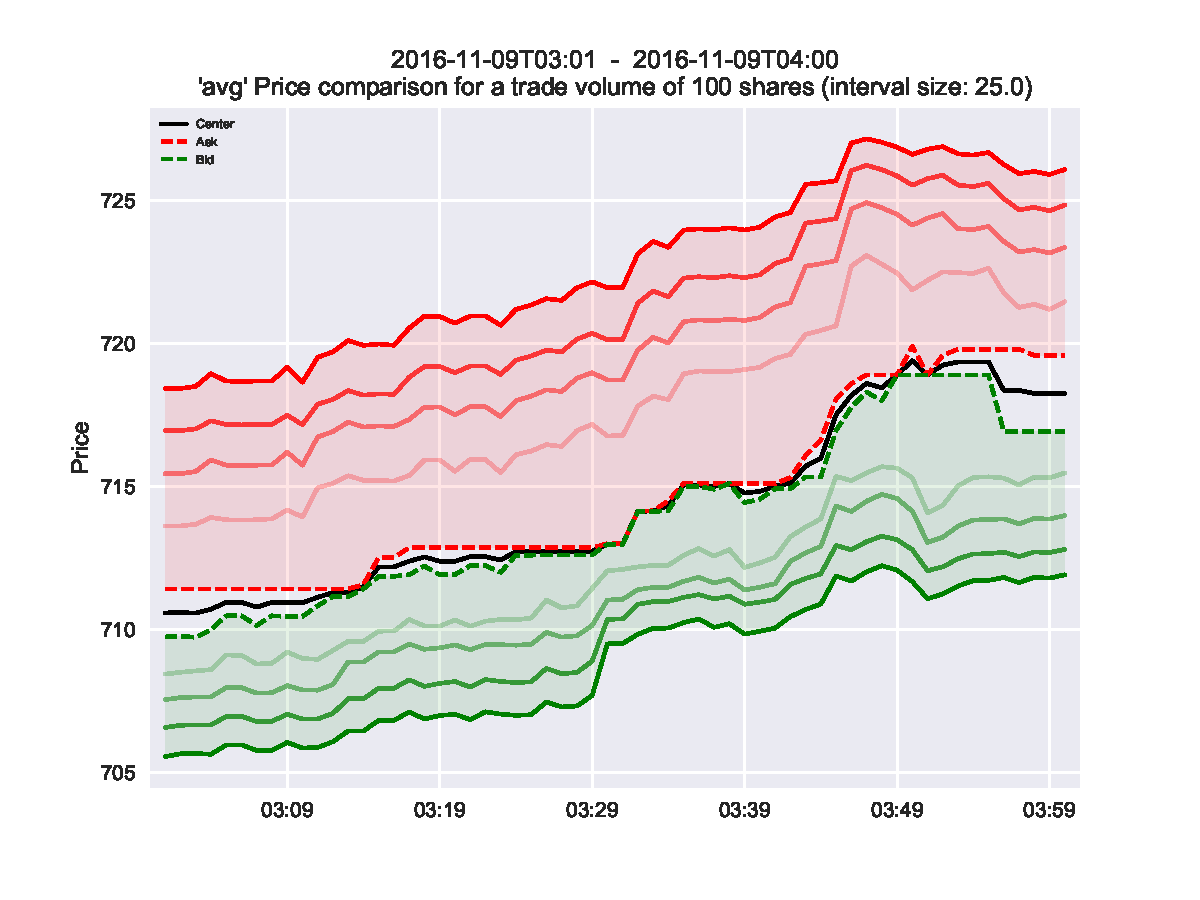
\includegraphics[width=\textwidth]{content/drawings/orderbook_window17}
        		\caption{Average market price.}
		\label{fig:orderbookwindow:avg}
    	\end{subfigure}%
	\begin{subfigure}[t]{0.5\textwidth}
        		\centering
        		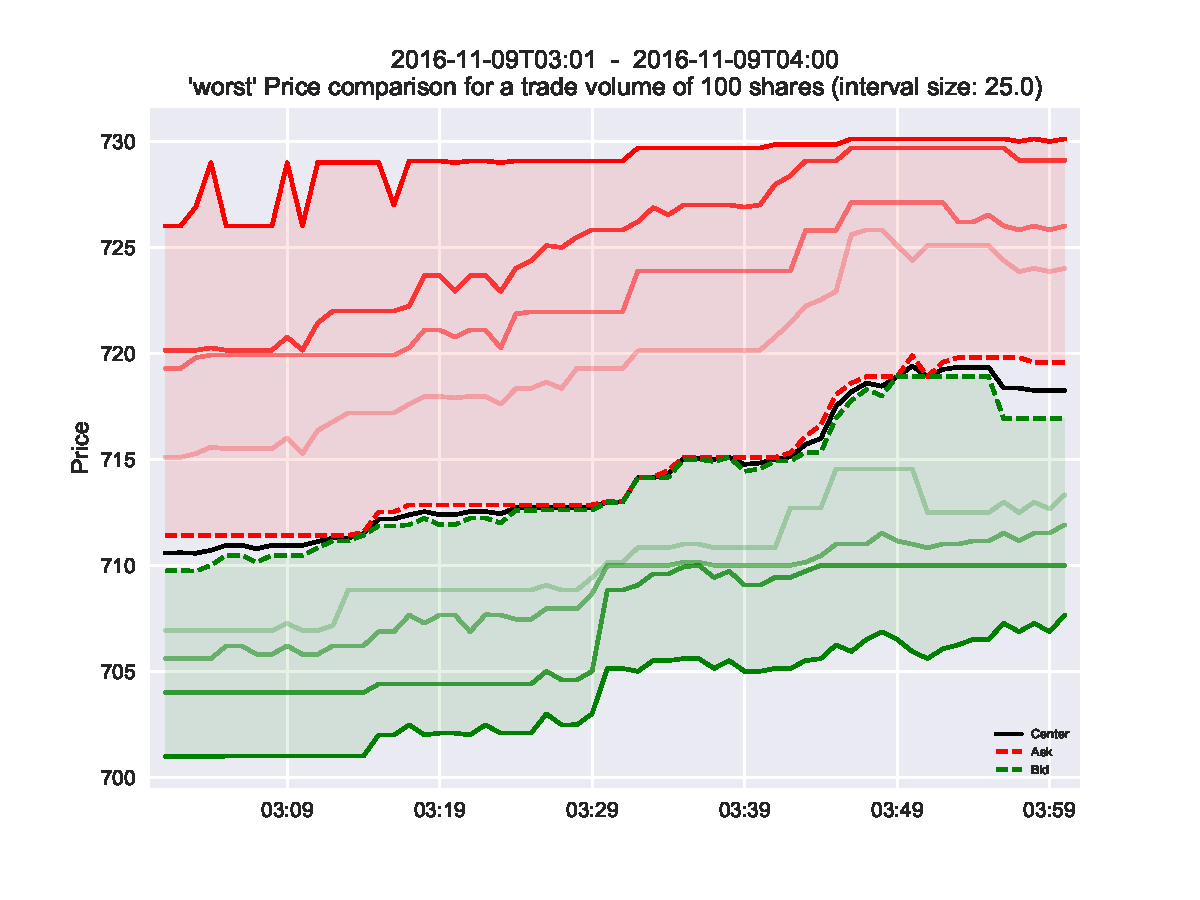
\includegraphics[width=\textwidth]{content/drawings/orderbook_window17_worst}
        		\caption{Worst market price.}
		\label{fig:orderbookwindow:worst}
    	\end{subfigure}%
	
	\caption{An orderbook window over a period of 60 minutes.}
	\label{fig:orderbookwindow}
\end{figure}

\subsection{Masterbook}
During instantiation, the \ac{OTS} creates a copy of the first orderbook, called the \emph{masterbook}. Hereinafter executed trades do only affect this internal \emph{masterbook}. The remaining orderbooks are then converted into \emph{deltabooks}, containing only changes between subsequent orderbooks.\\

The \ac{OTS} may be reset to its initial state at any time via \lstinline!ots.reset()!. This avoids computational overhead, when testing out multiple strategies on the same \emph{window}, as only \emph{masterbook} and \emph{history} are reset, while \emph{deltabooks} need not be recomputed and \emph{orderbooks} need not be retransferred. \lstinline!ots.reset()! provides optional parameters for modifying the simulators start conditions. As such the simulator might be instructed to start at a \lstinline!custom_starttime! or with a \lstinline!custom_startvolume!, to simplify the exploration of possible strategies.

\subsection{Trade execution}
\label{chap:tradeexecution}
The simulated trade execution is triggered by an external call to \lstinline!trade(limit=...)!. The \ac{OTS} expects a \lstinline!limit! and iterates over the next \lstinline!period_length! orderbooks, matching all eligible orders. The \lstinline!limit! represents the highest accepted price level for buy orders and the lowest accepted price level for sell orders respectively. If \lstinline!limit=None!, a simple market order is performed.\\

In a first step, all eligible orders, bound by the given limit and the total trade\_volume, are cut from the internal masterbook and pasted into the \lstinline!ots.trade_history!, as such these orders are assumed be fulfilled. The \lstinline!volume! and \lstinline!cash! variables are updated accordingly.
The simulator then moves to the next time point and adds the corresponding \emph{deltabook} to the masterbook.\\

In case of order size reductions\footnote{order size may be reduced, due to order fulfillment, order updates or order cancelations through the other market participants}, negative order sizes may appear in the masterbook. They are silently dropped, assuming they where matched before they actually vanished from the market. This is a possible source of trouble, as this assumption can not be proven to be valid. As such, matching orders that are simultaneously updated to another price level, are virtually doubled. They are perceived as a new order, even though the responsible market participant has already realized an execution and no basis to submit another one.\\

\begin{figure}[ht]
	\centering
	\begin{enumerate}
	\item \lstinline!master += diff(ob[t] - ob[t-1])!, drop negative share counts.
	\item perform trade: buy until given limit
	\item \lstinline!master -= bought bitcoins!
	\item done if \lstinline!volume==0! or $t==T-1$ (\lstinline!forced=True! a)
	\end{enumerate}
	\caption{Figure describing the masterbook adjustments as a graph?!}
	\label{fig:masterbookadjustments}
\end{figure}

The masterbook is then ready to be queried again. Any eligible \emph{new} orders are cut from the masterbook and past into the \lstinline!ots.trade_history!. After \lstinline!period_length! steps, a detailed trading report, as shown in \Cref{tab:tradinghistory} is returned. The upper case columns represent internal variables and orderbook statistics observed at the particular period start. The lower case columns summarize the actual trade in terms of highest, lowest and average price achieved, traded volume and cash and observed costs.\\

\begin{table}
\centering
\scalebox{0.44}{
\begin{tabular}{lrrrrrrrrrrrrlrrrr}
\toprule
{} &     ASK &     BID &  CENTER &  SPREAD &  LIMIT &   T &  VOLUME &  volume\_traded &      CASH &  cash\_traded & ... &     avg & forced &  initialMarketAvg &     low &    high &  cost \\
\midrule
03:01 &  711.42 &  709.74 &  710.58 &    1.68 &  713.0 &  15 &  100.00 &          46.77 &      0.00 &    -33280.72 & ... &  711.51 &  False &            718.42 &  711.42 &  713.00 &     43.48 \\
03:16 &  712.52 &  711.86 &  712.19 &    0.66 &  715.0 &  15 &   53.23 &          28.90 & -33280.72 &    -20630.99 & ... &  713.99 &  False &            718.42 &  712.52 &  715.00 &     98.53 \\
03:31 &  715.10 &  712.98 &  714.04 &    2.12 &  717.5 &  15 &   24.33 &           6.68 & -53911.71 &     -4780.95 & ... &  716.16 &  False &            718.42 &  715.10 &  717.41 &     37.28 \\
03:46 &  718.60 &  717.77 &  718.18 &    0.83 &  720.0 &  15 &   17.65 &          17.65 & -58692.66 &    -12706.15 & ... &  719.73 &  False &            718.42 &  718.60 &  720.00 &    161.57 \\
\bottomrule
\end{tabular}}
\caption{Trading history, as returned after four consecutive calls of \lstinline!ots.trade()!.}
\label{tab:tradinghistory}
\end{table}

\subsection{Visualization}
A visual representation of the same trading strategy, which underlies \Cref{tab:tradinghistory}, is shown in \Cref{fig:tradingstrategy17good}. Here, the \ac{OTS} was instructed to buy 100 bitcoins within a period of 60 minutes and called with four consecutive limits prices 713, 715, 717.5 and 720, which are shown as grey step function in the upper subplot.\\

The second subplot displays trade executions and declining trade volume over time and the bottom subplot displays induced costs. Expected costs conform to the respective accumulated costs, extrapolated to the full trade volume.

\begin{figure}[ht]
	\centering
   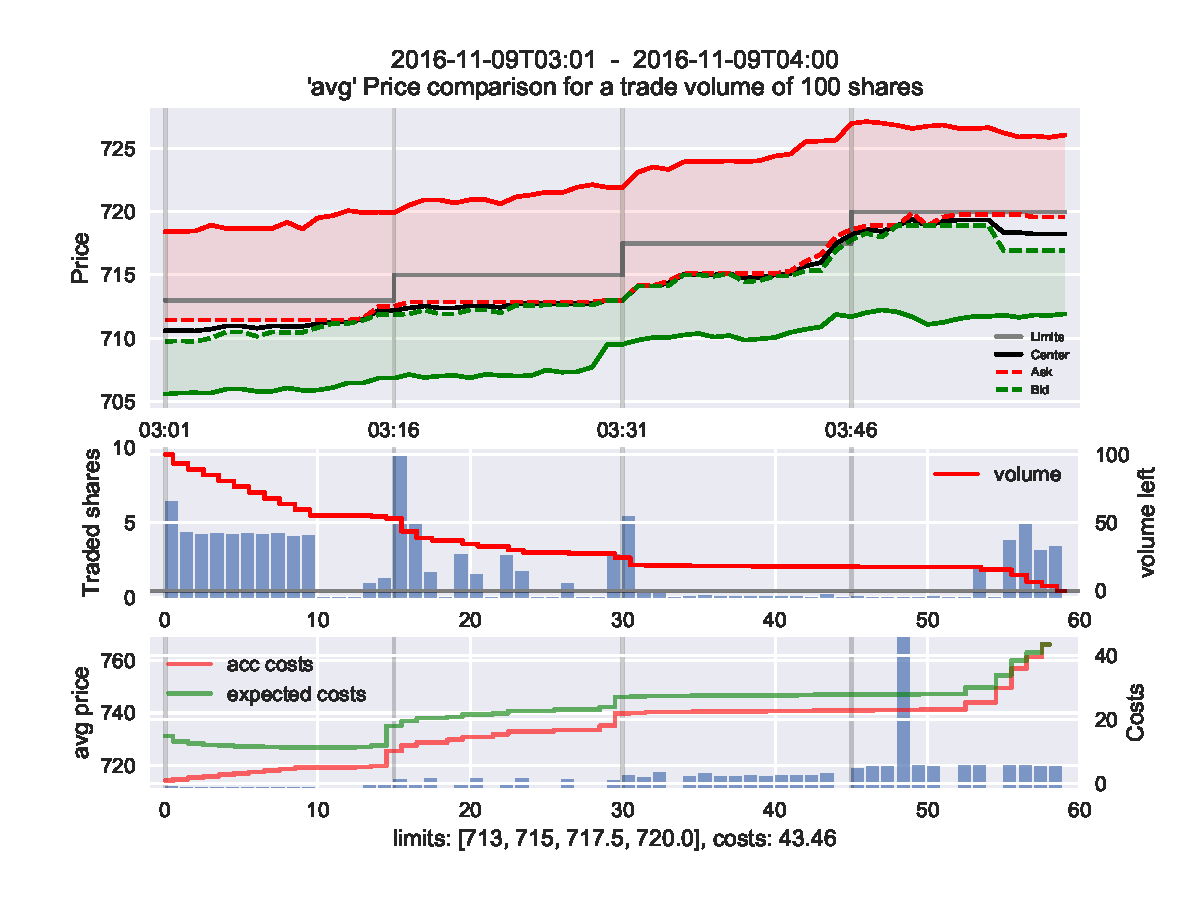
\includegraphics[width=0.8\textwidth]{content/drawings/trading_example17_good}
	\caption{Visualization of an exemplary trading strategy.}
	\label{fig:tradingstrategy17good}
\end{figure}

\subsection{Model correctness}
\label{chap:modelcorrectness}
The presented model does not account for market reactions, induced by the currently executed trading strategy. It moronically follows the market trend, as it would have evolved without any intervention. Some sources of troubles are pictures below:

\begin{itemize}
\item As stated in \Cref{chap:tradeexecution}, the presented model can not distinguish between a limit order being removed from the market makers orderbook and a limit order essentially only being updated to another price level. In the latter case, the order presumably wouldn't have reappeared in the orderbooks after the simulator matched it.
\item Other market participants typically monitor market activity thoroughly, which is particularly true for purely electronic markets of digital assets, like bitcoins. It is delusive to assume, that no other market participants or trading bots react to large orders, that eat significantly into the orderbook.\\

\begin{figure}[ht]
	\centering
	[placeholder]
	\caption{Sample of a \emph{curious masterbook shape}.}
	large part of order fulfilled, eaten deeply into the orderbook, deltabook brings in new orders close to original centerprice $\Rightarrow$ uncommon gap.
	\label{fig:masterbook:curiousshape}
\end{figure}

\item Orderbooks on a minutely basis miss a great part of the markets volatility. \\
In addition to orderbook snapshots, professional data providers typically grant access to market level 2 data (see \Cref{sec:marketdata:levels}) in form of log files as well. The log files consist of timestamped orderbook updates (typically of type \emph{remove} and \emph{modify}), which allow the reconstruction of the orderbook for an arbitrary time point. As mentioned in \Cref{chap:dataorigin}, Poloniex push API, to receive live order book updates and trades, was rather error-prone and occasionally failed to report important orderbook updates. As the valid reconstruction of orderbooks is highly vulnerable to missing logs, inconsistencies arose and the decision was made, to query orderbooks on a minutely basis only.
\item Hidden Orders, as introduced in \Cref{chap:ordertypes}, are not accounted for.
\end{itemize}

As a consequence, trading on the masterbook can only be seen as an rough approximation of true market behaviour. Curious masterbook shapes, resulting from the described simulation process, encourage to perform actual feature extraction on the original orderbooks, examining the market as it would have evolved without any interventions.







\cleardoublepage{}